\documentclass[12pt]{spieman}  % 12pt font required by SPIE;
%\documentclass[a4paper,12pt]{spieman}  % use this instead for A4 paper
\usepackage{amsmath,amsfonts,amssymb}
\usepackage{graphicx}
\usepackage{setspace}
\usepackage{tocloft}
\usepackage{lineno}
\linenumbers
\title{Supplemental Materials for "Machine Learning-Based Partition Function Sampling: Application to Fe on MgO(001) Growth"}

\author[a]{Andi Muhammad Nur Fitrah Syamsul}
\author[a]{Kohji Nakamura}
%\author[b]{Third Author}
%\author[a,b,*]{Fourth Author}
\affil[a]{Graduate School of Engineering, Mie University, Tsu, Mie 514-8507}
%\affil[b]{Company Name, Street Address, City, Country}

\renewcommand{\cftdotsep}{\cftnodots}
\cftpagenumbersoff{figure}
\cftpagenumbersoff{table} 
\begin{document} 
\maketitle

% Include a list of up to six keywords after the abstract
% \keywords{Crystal structure, Island growth, Fe/MgO, Machine learning}

% Include email contact information for corresponding author
{\noindent \footnotesize\textbf{*}Andi Muhammad Nur Fitrah Syamsul,  \linkable{andimuhammad164@gmail.com} }

\begin{spacing}{2}   % use double spacing for rest of manuscript

\newpage

\section{Computational Implementation}

The minimum-ensemble sampling process is executed using the Atomistic Global Optimization X (AGOX) python package \cite{Christiansen2022}. Within this package, the Global Optimization with First-principles Energy Expression (GOFEE) framework manages the interplay between the machine-learned Gaussian Process Regression (GPR) model and the first-principles evaluator. All underlying energy evaluations required for training the GPR model are performed using density functional theory (DFT) as implemented in the GPAW code \cite{jussi2010, Mortensen2024}.

\section{AGOX Environment}

The AGOX environment models the Fe-on-MgO system for the sampling process under specific structural constraints, as illustrated in Fig. \ref{Fig_env}: the substrate, consisting of Mg (orange) and O (red) atoms, is held fixed, while the Fe atoms (green) are subject to GPR optimization. To restrict the sampling effectively, we impose a boundary condition represented by the red box; the Fe atoms are confined within these lateral dimensions, while the height of the box along the $z$-axis is set to $8.4\text{ \AA}$. This volume defines the degrees of freedom for the Fe atoms, establishing the spatial limits within which they can rearrange during the optimization process to explore the Potential Energy Surface (PES).

\section{DFT Calculation}

The DFT calculations utilize the Perdew-Burke-Ernzerhof (PBE) exchange-correlation functional \cite{Perdew1996} and a linear combination of atomic orbitals (LCAO) basis set. To account for the ferromagnetic nature of the Fe islands, all DFT calculations are conducted with spin polarization. The surface Brillouin zone of the $5\times5$ supercell, which contains 25 atoms of each species, is sampled using a $1\times1$ k-point grid. High-order effects, specifically spin-orbit coupling and van der Waals interactions, are omitted from the search.

\section{Finite-Size Effects}

To evaluate the influence of finite-size effects on this motif, the island growth mode characteristics were tested against lateral constraints using reduced supercell dimensions of $3\times3$ (9 atoms per species) and $4\times4$ (16 atoms per species). As shown in Figure \ref{Fig_sup}, the consistent emergence of non-planar structures confirms that the island growth mode is a robust feature independent of supercell size, although the island height increases by approximately $1\text{ \AA}$ per area increment. This scaling behavior indicates that increased surface area facilitates the formation of taller Fe clusters to maximize bulk-like metallic bonding while minimizing interfacial contact energy.

\section{MgO-on-Fe}

A reverse deposition test was performed by modeling MgO-on-Fe growth to examine the directional dependence of the interface morphology. As shown in the inset of Fig. \ref{Fig_mgo}b, the ground state for this inverse configuration is a flat mode, contrasting the island mode observed for Fe-on-MgO. This result is consistent with experimental observations from Ref. \cite{ernult2003}, where molecular beam epitaxy (MBE) was utilized to grow single-crystalline MgO layers on Fe(001) electrodes. Their reflection high-energy electron diffraction (RHEED) characterization demonstrated that the MgO film maintains structural flatness and sharp diffraction streaks, supporting the identification of the flat mode as the preferred thermodynamic ground state. Furthermore, the temperature-dependent Boltzmann probability distribution (Fig. \ref{Fig_mgo}c) indicates that this flat ground state remains the dominant configuration even at elevated temperatures, confirming its high thermal stability.

%%%%% References %%%%%

\bibliography{report}   % bibliography data in report.bib
\bibliographystyle{spiejour}   % makes bibtex use spiejour.bst

\newpage

% \begin{figure}
% \begin{center}
% \begin{tabular}{c}
% 
\includegraphics[height=8.5cm]{figs/v6/Fig_flow.png}
% \end{tabular}
% \end{center}
% \caption 
% { \label{Fig_flow} Flowchart of the modified GOFEE iteration framework, detailing the biased exploration strategy.} 
% \end{figure} 

\begin{figure}
\begin{center}
\begin{tabular}{c}
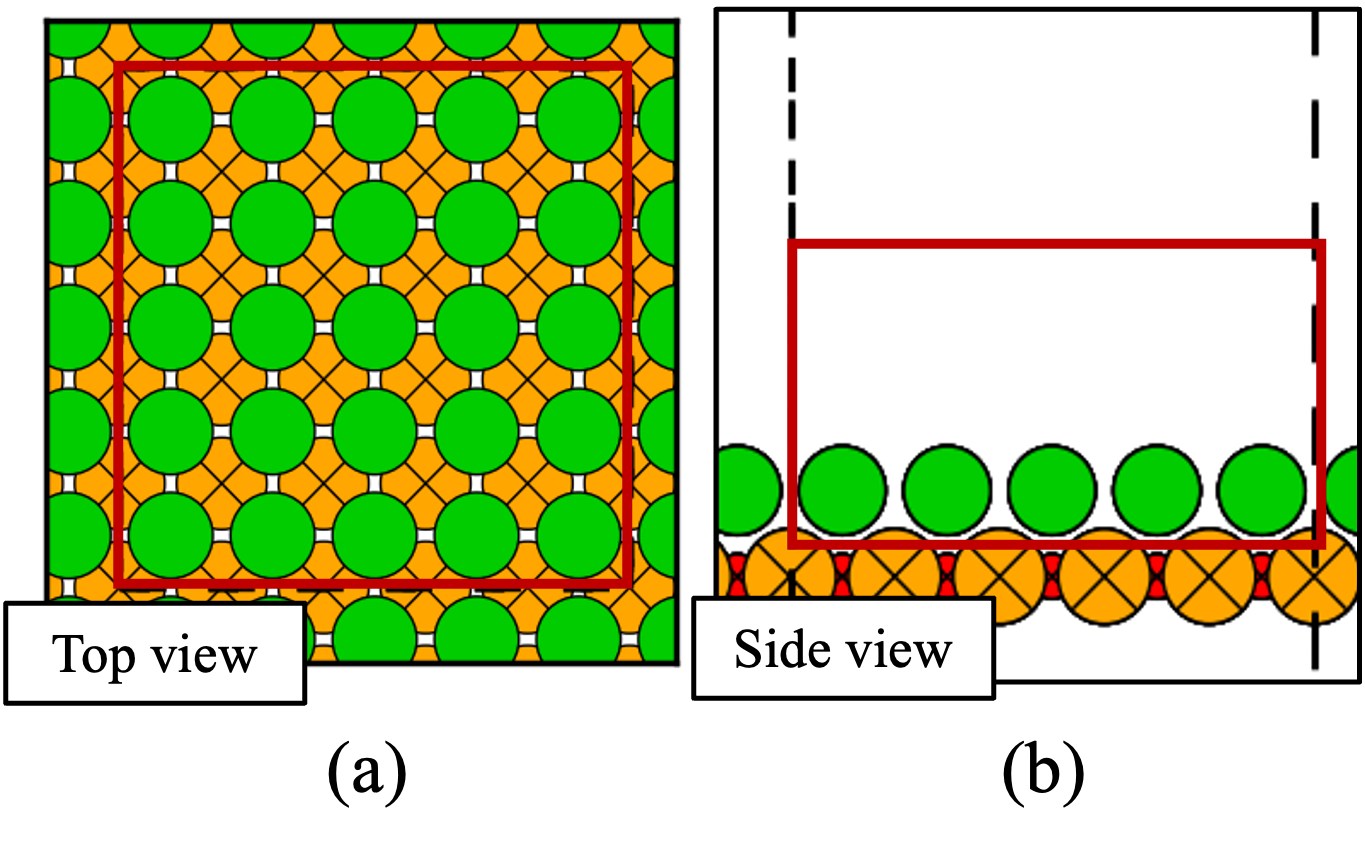
\includegraphics[height=7.5cm]{figures/Fig_env.png}
\end{tabular}
\end{center}
\caption 
{ \label{Fig_env} Schematic representation of the AGOX environment for the Fe-on-MgO system. (a) Top view and (b) side view illustrate the atomic species: Fe (green), Mg (orange), and O (red). The dashed lines indicate the periodic boundaries, while the red box signifies the GPR optimization constraint, defining the allowed range of motion for the mobile Fe atoms. The $z$-axis height of this constraint box is set to 8.4 Å. Crossed-out atoms (Mg and O) denote the fixed substrate components.} 
\end{figure} 

\begin{figure}
\begin{center}
\begin{tabular}{c}
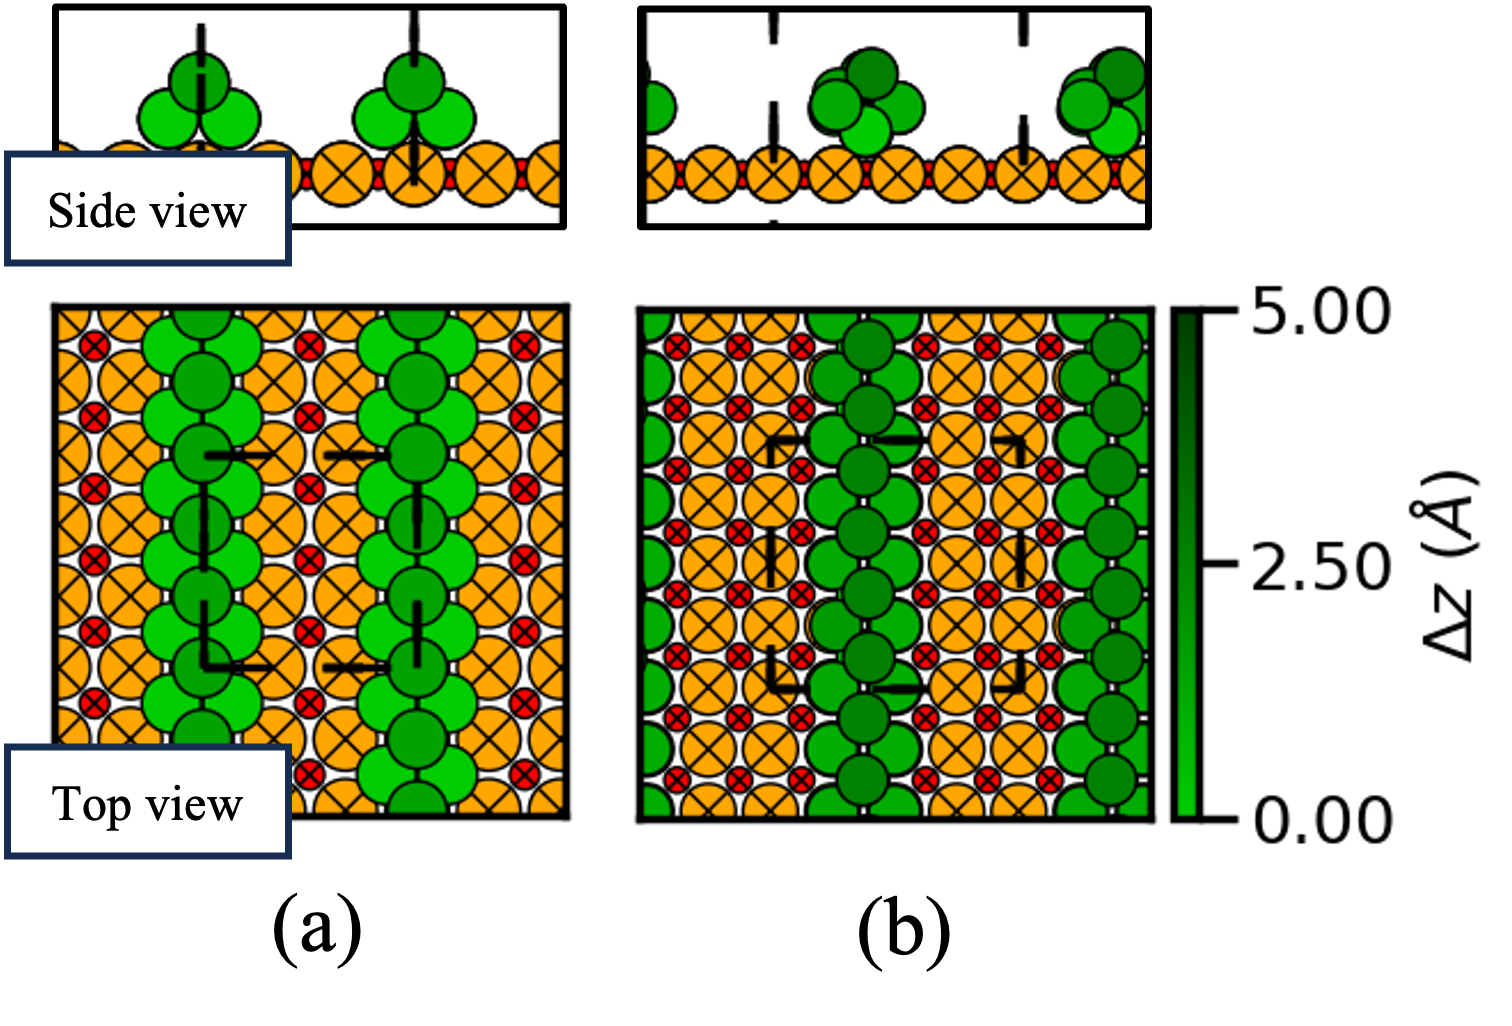
\includegraphics[height=8.5cm]{figures/Fig_sup.png}
\end{tabular}
\end{center}
\caption 
{ \label{Fig_sup} Ground-state configurations of $\text{Fe}$ (green spheres) on top of the underlying $\text{MgO(001)}$ monolayer substrate (orange and red spheres) for the (a) $3\times3$ and (b) $4\times4$ supercells. The dashed outlines demarcate the periodic boundaries of the respective supercells.} 
\end{figure} 

\begin{figure}
\begin{center}
\begin{tabular}{c}
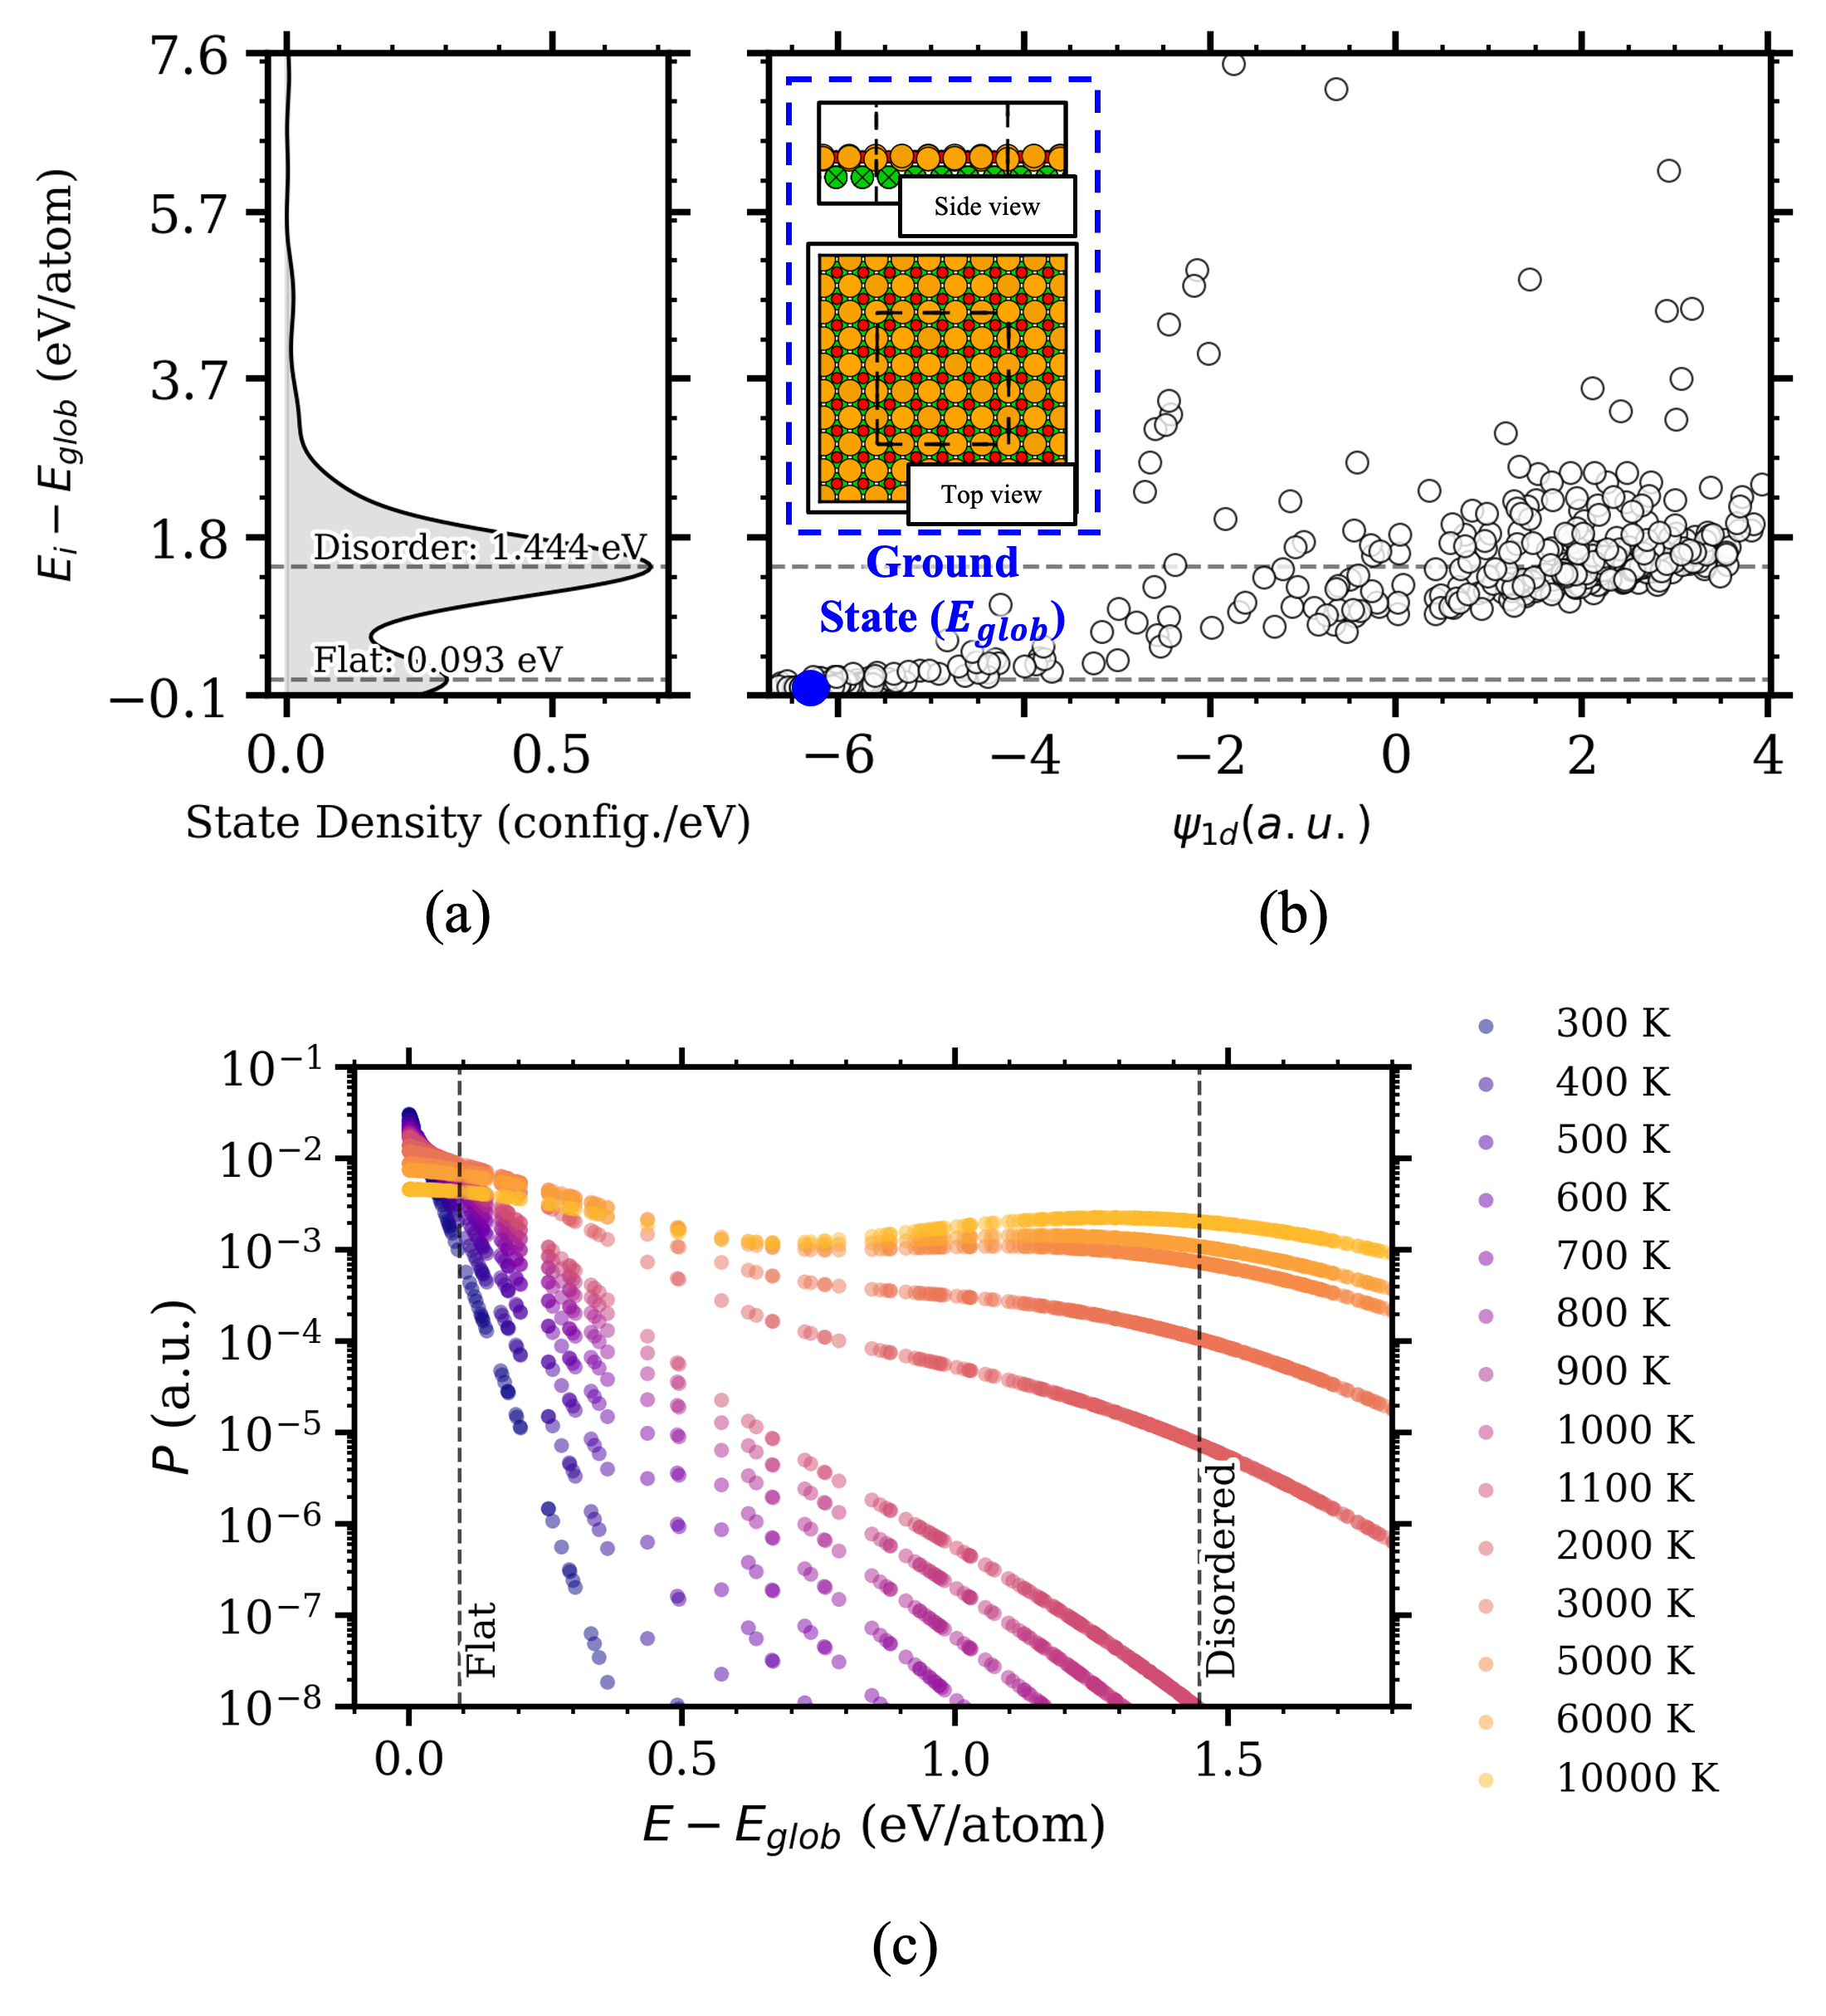
\includegraphics{figures/Fig_mgo.png}
\end{tabular}
\end{center}
\caption 
{ \label{Fig_mgo} Reverse deposition test for an $\text{MgO}$ monolayer on an $\text{Fe(001)}$ substrate. (a) The continuous state density distribution $g(E)$ and (b) the structural landscape mapped using the first principal component ($\psi_{1d}$) from the eigenvalue composition of the Valle-Oganov descriptor \cite{valle2010}. (c) The temperature-dependent Boltzmann density $\rho_B(E)$ (normalized so that $\int \rho_B \, dE = 1$) for the reverse-deposition ensemble, indicating that the flat ground state remains the dominant configuration even at elevated temperatures.} 
\end{figure} 

% \begin{figure}
% \begin{center}
% \begin{tabular}{c}
% 
\includegraphics[height=8.5cm]{figs/v6/Fig_convStateDens.png}
% \end{tabular}
% \end{center}
% \caption 
% { \label{Fig_convStateDens} Comparison of the state density distribution $g(E)$ obtained from a single GOFEE run (seed 0, black line) against cumulative distributions formed by sequentially aggregating independent runs from seed 0 up to seed 13 (shades of blue).} 
% \end{figure} 

% \begin{figure}
% \begin{center}
% \begin{tabular}{c}
% 
\includegraphics[height=8.5cm]{figs/v6/Fig_category.png}
% \end{tabular}
% \end{center}
% \caption 
% { \label{Fig_category} K-means clustering analysis of the ensemble produced across all sampling, derived from the Oganov-Valle descriptor \cite{valle2010} using the first two principal components (PCA). (a) Two-dimensional PCA projection mapping the structural landscape into 10 distinct categories (color-coded by Category ID), where PCA 1 and PCA 2 account for 69.1\% and 12.7\% of the total structural variance, respectively. (b) Statistical energy distribution ($E_i - E_{\text{glob}}$) corresponding to each identified cluster category. This analysis, which is included within the AGOX package, was used on the large-scale generator to ensure diversity during the generation process.} 
% \end{figure} 

%%%%% Figures %%%%%

% \begin{figure}
% \begin{center}
% \begin{tabular}{c}
% \includegraphics[height=8.5cm]{figs/v4/fig2_gofee.png}
% \end{tabular}
% \end{center}
% \caption 
% { \label{fig:gofee} The workflow of the GOFEE algorithm as implemented within the AGOX package. The algorithm is composed of three primary components: Structure Preparation, ML Relaxation, and Active Learning. The Structure Preparation uses a Structure Database for storage, where K-means Clustering is applied to select a diverse population for effective sampling. A Structure Generator produces new candidate configurations by applying stochastic operations such as rattling. The ML Relaxation component performs local optimization based on energy and uncertainty predictions provided by a Gaussian Process Regression (GPR) surrogate model on generated candidates. An LCB (Lower Confidence Bound) Acquisition function is then used to select the most promising structure, prioritizing configurations with low predicted energy or high predictive uncertainty. The Active Learning component performs a DFT evaluation to obtain the target potential energy of the selected structure, which is then used for GPR training to update the surrogate model for subsequent iterations.} 
% \end{figure} 

% \begin{figure}
% \begin{center}
% \begin{tabular}{c}
% \includegraphics[height=8.5cm]{figs/v4/fig1_ref.png}
% \end{tabular}
% \end{center}
% \caption 
% { \label{fig:ref} (a) shows the $zx$ view of the MgO/Fe(001)-($3 \times 3$) reference structure, where the interlayer distance is set at 2.3 Å. (b) displays the $xy$ view of the reference structure, utilizing an optimized Fe lattice constant of 2.87 Å. The MgO layer is rotated 45° in-plane to position the oxygen and Fe atoms directly atop one another. (c) shows the MgO/Fe(001) scheme in which the Fe substrate is constrained while the MgO acts as a free layer during structural relaxation. (d) shows the Fe/MgO(001) scheme, where the MgO is fixed, and the Fe layer is permitted to relax.} 
% \end{figure} 

% \begin{figure}
% \begin{center}
% \begin{tabular}{c}
% \includegraphics[height=6.5cm]{figs/v4/fig3_structGen.png}
% \end{tabular}
% \end{center}
% \caption 
% { \label{fig:structGen} A rattle mutation is applied to generate a new candidate. Within the REFERENCE structure, atoms denoted with a cross are constrained during generation, while those without a cross represent free atoms available for displacement. Two types of rattle algorithms were used: RATTLE 1, which applies a 1.5 Å maximum displacement to all free atoms, and RATTLE 2, which applies a 2.5 Å maximum displacement to half of the free atoms. To manage the search progression, an ITERATION GENERATION CONTROL scheme is implemented to generate 20 candidate structures in each search iteration. During iterations 0 through 9, all candidates are generated via RATTLE 1; starting from the 10th iteration, the population is divided equally with 10 structures each from RATTLE 1 and RATTLE 2; and following the 25th iteration, all 20 candidates are generated using the RATTLE 2 operation to promote further exploration.} 
% \end{figure} 

% \begin{figure}
% \begin{center}
% \begin{tabular}{c}
% \includegraphics[height=8.5cm]{figs/v4/fig5_result.png}
% \begin{picture}(0,0)
% \put(-300,-10){\small (a)}
% \put(-80,-10){\small (b)}
% \end{picture}
% \end{tabular}
% \end{center}
% \caption 
% { \label{fig:eProg} a) shows the energy progression during the search for the lowest energy structure ($E_{glob}$), where the y-axis shows the energy difference between each structure and the global minimum, normalized by the number of atoms in the system ($E_{rel}$). The x-axis indicates the cumulative number of structures incorporated into the GPR training dataset, demonstrating the model's increasing capability to identify the $E_{glob}$ as more data is acquired. Red squares provide snapshots of relaxed structures throughout the search iterations until the $E_{glob}$ is reached. b) illustrates the state density of generated candidate structures across $E_{rel}$. To achieve a smooth approximation of the underlying state density, a one-dimensional kernel density estimate (KDE) with a Gaussian kernel was fitted to the distribution of candidates.} 
% \end{figure} 

% \begin{figure}
% \begin{center}
% \begin{tabular}{c}
% \includegraphics[height=8.5cm]{figs/v4/fig6_globMin.png}
% \end{tabular}
% \end{center}
% \caption 
% { \label{fig:glob} The atomic configurations corresponding to the $E_{glob}$ identified through the GOFEE iterations for the 1 ML and 2 ML systems. These configurations highlight the structural favorability of both the MgO/Fe and Fe/MgO schemes at these thicknesses.} 
% \end{figure} 

% \begin{figure}
% \begin{center}
% \begin{tabular}{c}
% \includegraphics[height=10.6cm]{figs/v4/fig7_minE.png}
% \end{tabular}x
% \end{center}
% \caption 
% { \label{fig:local} The atomistic configurations corresponding to the local minima for the (1 ML) Fe/MgO schemes. These configurations are arranged in a hierarchy based on their $E_{rel}$ in meV/atom, depicting structural variations with respect to the most stable structure found during the search.} 
% \end{figure} 

%%%%%%%%%%%%

% \begin{figure}
% \begin{center}
% \begin{tabular}{c}
% 
\includegraphics[height=8.5cm]{figs/v5/Fig_Prog.png}
% \begin{picture}(0,0)
% \put(-300,-10){\small (a)}
% \end{picture}
% \end{tabular}
% \end{center}
% \caption 
% { \label{fig:eProg} shows the energy progression during the search for the lowest energy structure ($E_{glob}$), where the y-axis shows the energy difference between each structure and the global minimum, normalized by the number of atoms in the system ($E_{rel}$). The x-axis indicates the cumulative number of structures incorporated into the GPR training dataset, demonstrating the model's increasing capability to identify the $E_{glob}$ as more data is acquired.} 
% \end{figure} 

% \begin{figure}
% \begin{center}
% \begin{tabular}{c}
% 
\includegraphics[height=8.5cm]{figs/v5/Fig_ConDen.png}
% \end{tabular}
% \end{center}
% \caption 
% { S\label{FigConDis}} 
% \end{figure} 

% \begin{figure}
% \begin{center}
% \begin{tabular}{c}
% 
\includegraphics[height=8.5cm]{figs/v5/Fig_Boltz.png}
% \end{tabular}
% \end{center}
% \caption 
% { \label{FigProb}} 
% \end{figure} 

% \begin{figure}
% \begin{center}
% \begin{tabular}{c}
% \includegraphics[height=8.5cm]{figs/v5/Fig_DenHeight.png}
% \end{tabular}
% \end{center}
% \caption 
% { \label{FigZDist}} 
% \end{figure} 

% \begin{figure}
% \begin{center}
% \begin{tabular}{c}
% \includegraphics[height=8.5cm]{figs/v5/Fig_flowGoff.png}
% \end{tabular}
% \end{center}
% \caption 
% { \label{fig:flow}} 
% \end{figure} 

% \begin{figure}
% \begin{center}
% \begin{tabular}{c}
% \includegraphics[height=7.5cm]{figs/v5/Fig_Sup.png}
% \end{tabular}
% \end{center}
% \caption 
% { \label{fig:supercells} The atomic configurations corresponding to the supercell configurations of Fe on MgO(001) systems.} 
% \end{figure} 

% \begin{figure}
% \begin{center}
% \begin{tabular}{c}
% \includegraphics[height=8.5cm]{figs/v5/Fig_dos_5x5.png}
% \end{tabular}
% \end{center}
% \caption 
% { \label{fig:dos5x5}} 
% \end{figure} 

% \begin{figure}
% \begin{center}
% \begin{tabular}{c}
% \includegraphics[height=8.5cm]{figs/v5/Fig_Ground.png}
% \end{tabular}
% \end{center}
% \caption 
% { \label{fig:glob} The atomic configurations corresponding to the $E_{glob}$, or the ground-state configurations identified through the GOFEE optimization. These configurations highlight the structural favorability of both the MgO on Fe(001) and Fe on MgO(001) systems.} 
% \end{figure} 

\end{spacing}
\end{document}